%%%%%%%%%%%%%%%%%%%%%%%%%%%%%%%%%%%%%%%%%%%
%%%%%%%%%%%%%%%%%%%%%%%%%%%%%%%%%%%%%%%%%%%
%%%%%%%%%%%%%%%%%%%%%%%%%%%%%%%%%%%%%%%%%%%
\chapter{State of the Art}
\label{Sec:star}
In this chapter we will present the state of the art work present in bioinformatical literature with regards to the visualization and analysis of intermolecular interactions of proteins. We will start with overview of existing molecular visualization techniques, then continue with the work related to protein-ligand interactions, where literature covers a substantial amount of diverse research. Then we will continue with analysis of protein-protein interactions. This field is however only sparsely covered in literature.

\section{Molecular Visualization}
\subsection{Atomistic and Bond-Centric Models}
\begin{wrapfigure}{r}{0.3\textwidth} 
\vspace{-27pt}
  \begin{center}
  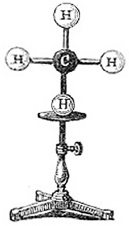
\includegraphics[width=0.9\linewidth]{pictures/04_hoffman.jpg} 
  \caption{Hoffman's methane (Marsh-gas) representation \cite{perkins2005history}.}
  \label{Fig:hoffman}  
\end{center}
  \vspace{-15pt}
\end{wrapfigure}

We can say that history of molecular visualization dates back to the 19th century. In 1808 John Dalton published his atomic theory~\cite{dalton1808new}, where he represented atoms and simple molecules with circular shapes. Couple of decades later, around 1860, August Wilhelm von Hoffmann started using first 3D models of molecules in his lectures at Royal Institution of Great Britain~\cite{perkins2005history} -- see Figure \ref{Fig:hoffman}. This type of molecular representation is called \textit{ball-and-stick} model, where balls represent atoms and sticks represent bonds between them. With couple of modifications this representation is commonly used also nowadays (Figure \ref{Fig:vis} b)). 

Over the years other derivations of ball-and-stick model emerged. In 1959 André Dreiding introduced molecular modelling kit using \textit{stick-only} model~\cite{dreiding1959einfache}. Here the atoms were not represented by balls, but merely as connection points between sticks. Nowadays this model is called also \textit{liquorice} or \textit{Dreiding's model} (Figure \ref{Fig:vis} a)). The colouring of the sticks is often used to indicate atoms or their properties.

Although several researchers, including Dalton and Hoffman, claimed that different atoms have different radii, it wasn't until 1873 that the sizes of atoms were experimentally derived by Johannes Diderik van der Waals~\cite{Waals1873PhDThesis}. In later years this discovery led to so called \textit{space-filling} molecular representations, also called \textit{callote} or \textit{CPK models} after chemists Robert Corey, Linus Pauling, and Walter Koltun \cite{corey1953molecular}. In this representation, full "space-filling" sizes of atoms are used, which provides the overview of molecular surface (Figure \ref{Fig:vis} c)).

\begin{figure}[H]
  \centering
  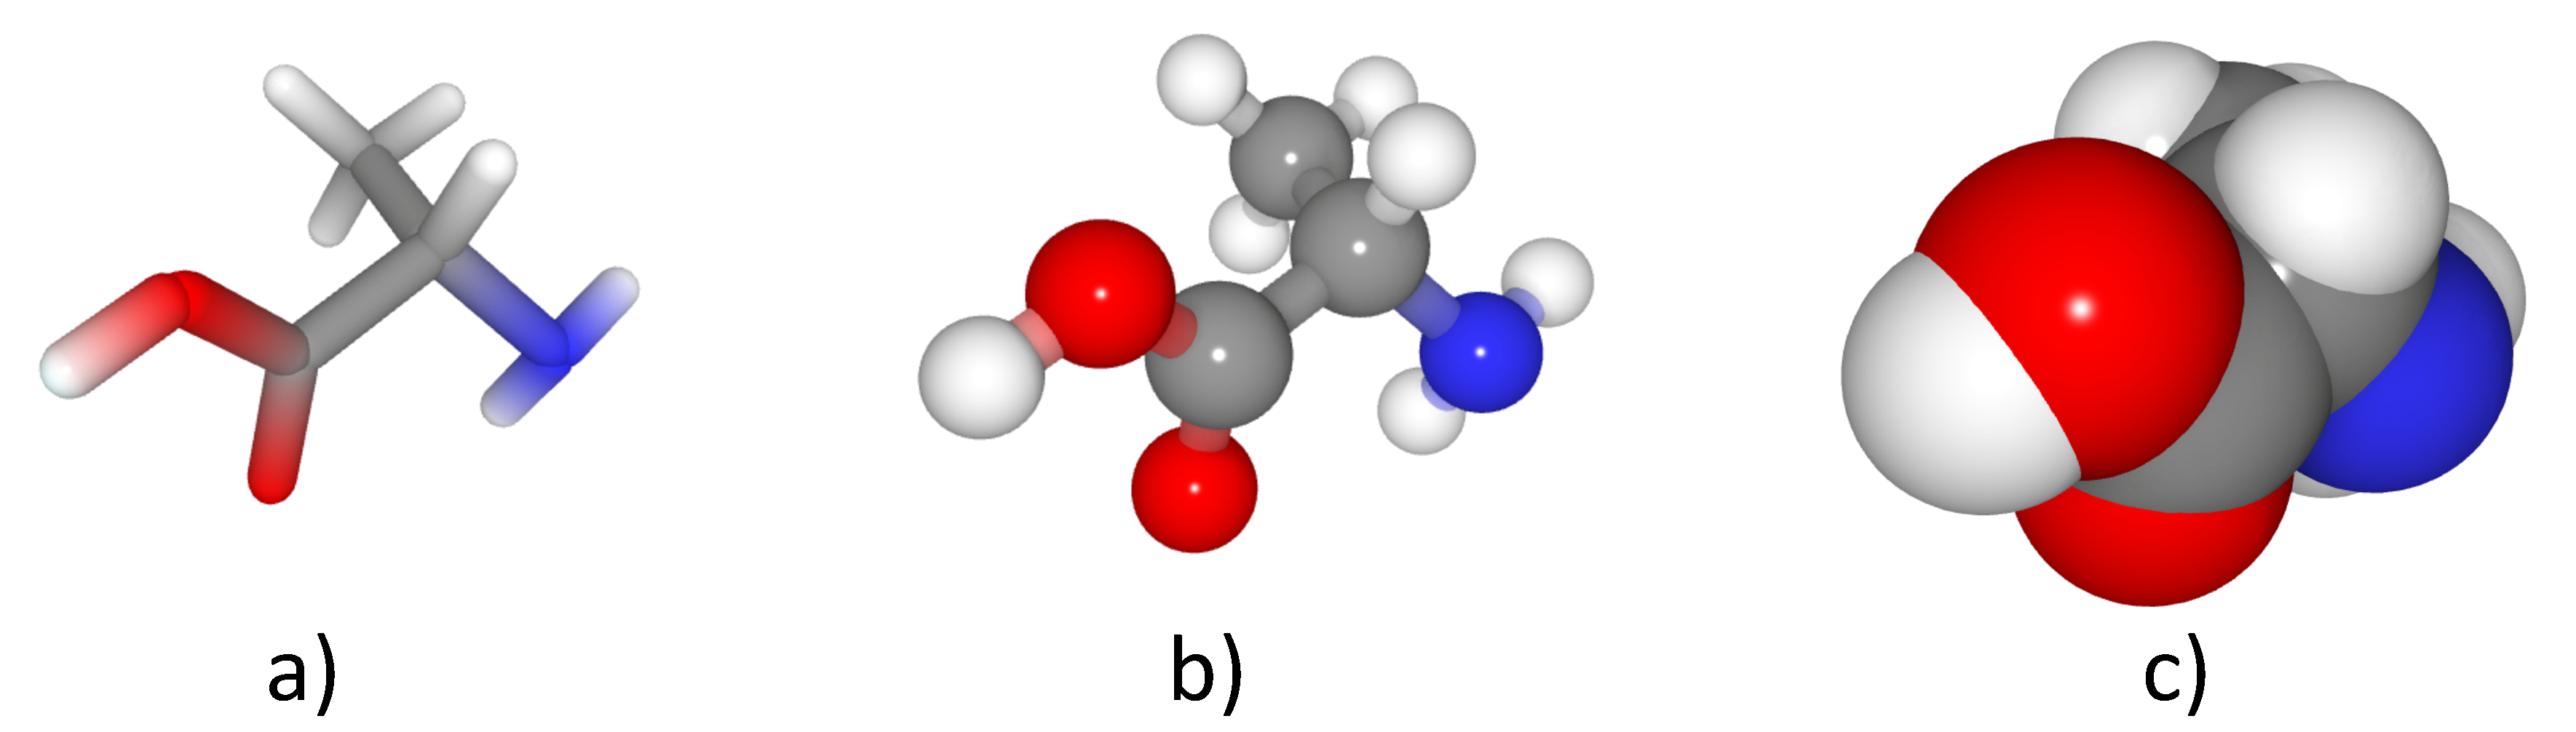
\includegraphics[width=\linewidth]{pictures/vis.pdf} 
  \caption{Types of molecular representations in modern visualization tools: a) liquorice model b) ball-and-stick model c) space-filling model}
  \label{Fig:vis}  
\end{figure} 

Atom and bond based representations of molecules can be decomposed into primitive shapes such as spheres and cylinders, which makes them suitable for GPU-based ray casting. Most of the state of the art rendering techniques stem from glyph ray casting introduce by Gumhold et al. \cite{gumhold2003splatting}, however many performance speedups focusing on rendering of large dynamic molecular structures exist. Since these techniques are focusing on large data samples, they often utilize level of detail (LOD) strategies. Example of this can be the two-level approach of Lampe et al. \cite{lampe2007two} where residues are each residue is represented by one vertex and the atoms in the residues are generated on-the-fly on the GPU. Another approach is used by Le Muzic et al. \cite{le2014illustrative}, where atom positions are stored in a texture and reconstructed using tessellation and geometry shaders.

\subsection{Protein Architecture}
The afore mentioned representations of molecules provide detail information about arrangement of atoms in a molecule. However, for proteins, which can consist of thousands of atoms, this representations can be too cluttered. Therefore, several schematic visualizations were developed.

One of the simplest representations of protein structure is called \textit{alpha trace}. It depicts only the backbone of the protein, as it is derived from the positions of $\alpha$-carbons (Figure \ref{Fig:vis2} a)). This representation provides coarse overview of tertiary and quaternary structure of the protein -- spatial arrangement of the polypeptide chains. However, it can be difficult to identify secondary structures from the alpha trace.

\begin{figure}[H]
  \centering
  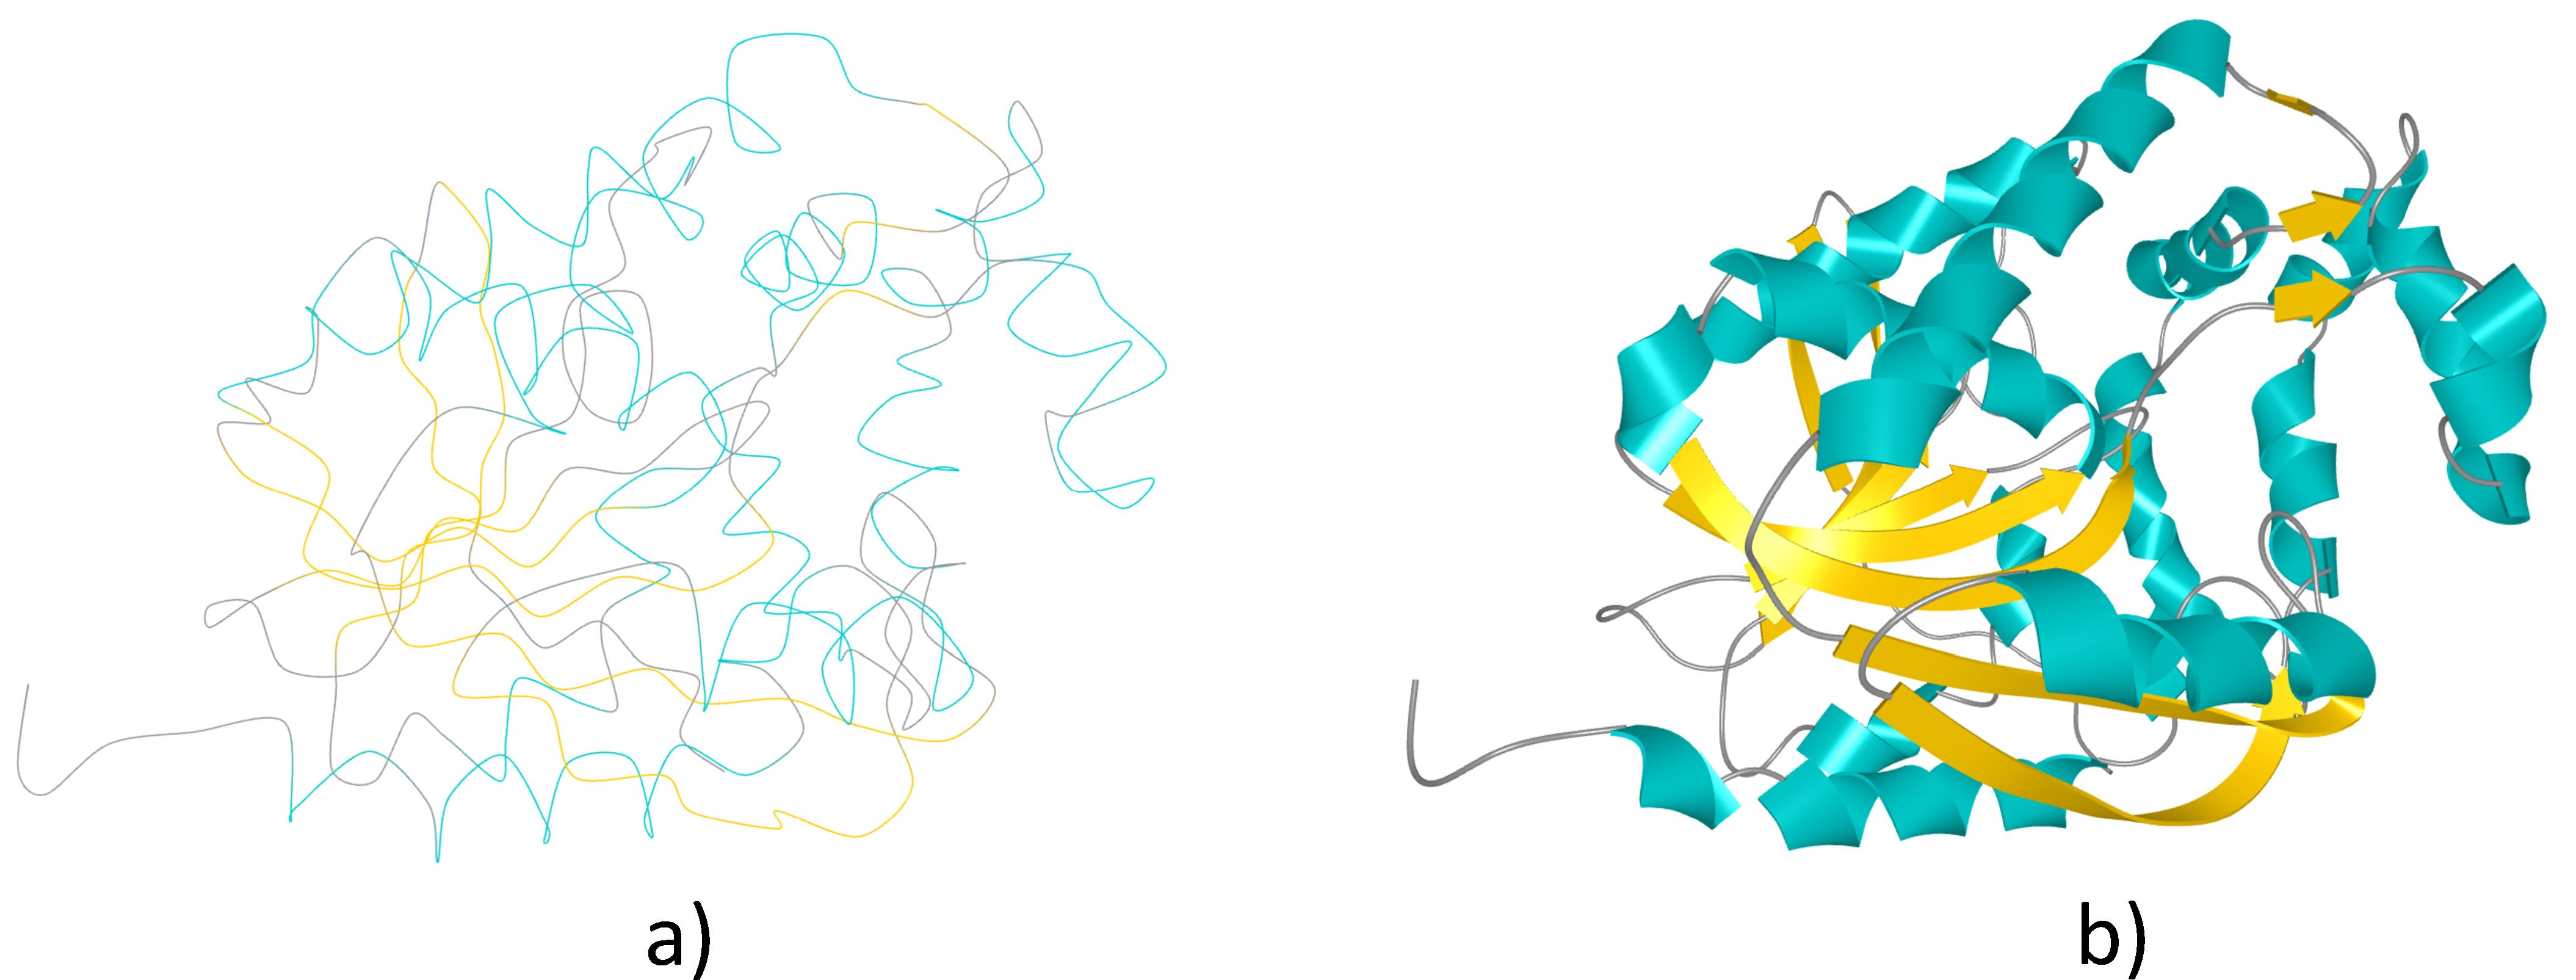
\includegraphics[width=\linewidth]{pictures/representations.pdf} 
  \caption{Types of molecular representations in modern visualization tools: a) alpha trace b) ribbon diagrams}
  \label{Fig:vis2}  
\end{figure} 

In 1981 Jane S. Richardson published \textit{cartoon} illustrations of all then known protein structures \cite{richardson1981anatomy}. In these schematic representations, known today as \textit{ribbon diagrams}, she used consistent and intuitive illustrations of secondary structures to demarcate their position along protein backbone. Although ribbon diagrams were originally hand drawn, they are nowadays part of every molecular visualization software (Figure \ref{Fig:vis2} b)).

\subsection{Surface Representations}
These representations communicate the internal structure of the protein. However in many cases the focus of interest is on the surface of the protein, since the surface is the part of protein that is in contact with outer environment. In is therefore important for biochemists to identify the boundaries of the proteins that are accessible to ligands or interacting with other proteins.

We have already mentioned one type of surface defined by atom spheres of van der Walls radii and therefore called \textit{van der Waals (vdW) surface} \cite{richards1977areas} -- Figure~\ref{Fig:surface} (blue). This surface indicates the precise molecular volume.

Another type of surface -- \textit{solvent accesible surface (SAS)} was developed to show the regions of molecule accesible by a solvent molecules \cite{lee1971interpretation}. Here, the solvent molecule is approximated by a spherical probe, which rolls rolls over the vdW surface. The center of the probe than defines the SAS surface -- Figure~\ref{Fig:surface} (yellow). In other words, solvent accesible surface is equal to a vdW surface inflated by the radius of probe.

\begin{figure}[htb]
  \begin{center}
  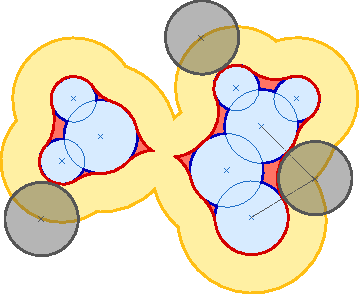
\includegraphics[width=0.5\linewidth]{pictures/surface.pdf} 
  \caption{Schematic representation of molecular surfaces: vdW surface (blue), SES (red) and SAS (yellow). The SES and SAS are defined a probe (grey) rolling over vdW surface. Image taken from \cite{kozlikova2015visualization}.}
  \label{Fig:surface}  
\end{center}
\end{figure}


\textit{Solvent excluded surface (SES)} \cite{richards1977areas} is defined in similar manner to SAS. However, instead of the center of the probe, its outer shell defines the surface -- Figure~\ref{Fig:surface} (red). It was the first smooth surface defined and thanks to the close approximation of molecular volume it is one of the most used surface representations. Many algorithms for its computation and visualization have been developed over the years. Currently the fastest soulutions include paralelization of contour-buildap algorithm \cite{totrov1996contour} -- algorithm that computes track of the probe on atom surfaces -- by Lindow et al. \cite{lindow2010accelerated} and Krone et al. \cite{6094043} as well as a grid-based approach by Hermosilla at al. \cite{hermosilla2017interactive} that utilizes progressive refinement for rendering of dynamic models on the fly.

Yet another type of molecular surface -- \textit{Molecular skin surface (MSS)} was proposed by Edelsbrunner \cite{edelsbrunner1999deformable}. The shape of MSS depends on the single parameter \textit{s} -- shrink factor. The advantage of MSS over SES is full $C^1$ continuity.  Among the fastest aproaches to generation of MSS belong the ones by Lindow et al. \cite{lindow2010accelerated} and \cite{Yan2017}.

\textit{Ligand exluded surface (LES)} is a relatively new generalization of SES proposed by Lindow et al. \cite{lindow2014ligand}. Instead of using an approximate probe, it uses full geometry of ligand to generate the surface. It thus illustrates the precise accessibility, however it is very computationally demanding.

In 1982 Blinn \cite{blinn1982generalization} proposed use of a Gaussian convolution
kernel to blend atom potentials to achieve an approximation of molecular surface. This technique is more commonly known as Metaballs. As with other techniques, improvements and new kernels have been proposed over the years (e.g. by Krone et al. \cite{krone2012fast}) and the resulting techniques belong to the fastest surface rendering approaches.

\begin{figure}[H]
  \centering
  \includegraphics[width=\linewidth]{pictures/surface2.pdf} 
  \caption{Comparison between different molecular surfaces of the protein isomerase: a) vdW surface b) SES with probe radius 1:4 Å c) LES for equilenine d) MSSwith shrink factor 0.35 e) Gaussian surface with standard deviation equal to the atom radius. Image taken from \cite{kozlikova2015visualization}.}
  \label{Fig:surface2}  
\end{figure} 

Note that we have only mentioned several state of the art techniques that deal with the representation of molecular surfaces. Examples of their results can be found in Figure \ref{Fig:surface2}. There are, however, countless of other approaches that exceed the capacity of this work.The detailed study concerning molecular representation can be found in state of the art report by Kozlikova et al. \cite{kozlikova2015visualization}. Available is also the report by Patané and Spagnuolo focusing on modeling of molecular surfaces.

Simplifications

Enhancemts


Molecular Visualization systems

enhancements - ao, depth,..., abstractions, tools (py mol, analyst)





star on molecular vis \cite{kozlikova2015visualization}
stra on surfaces \cite{patane2015state}

\section{Detection of Protein Voids}
As we mentioned before, the active site -- the reactive area of the protein is often buried deeply inside of the protein structure and accessible only via protein tunnels. Therefore extraction and analysis of these tunnels is vital for the study of protein-ligand binding. There are several methods for extracting the shape of the protein voids in general, as well as numerous ones focusing on tunnels specifically. The algorithms can be classified into several categories, depending on the approach they use: grid-based, probe-based, surface-based, Voronoi-based, ligand based and path analysis. Most of the algorithms combine several approaches, in order to achieve better results. Moreover, we can differentiate  between algorithms applicable only for static structures and algorithms taking into account molecular dynamics.

Due to the extensiveness of the work related to this topic, we will name only several representatives to demonstrate the basic principles of these approaches. Complete overview of the published tools for detection and analysis of biomolecular cavities can be found in state of the art reports by Krone et al. \cite{krone2016visual} and \cite{simoesgeometric}.
%In 2012 Berzovsky et. al. published the overview these tools \cite{brezovsky2013software}.

Many algorithms for void detection use a voxel grid to subdivide the 3D space containing the protein. An exaple of a \textbf{grid-based approach} that also utilizes \textbf{path analysis} is the first version of CAVER algorithm \cite{Petrek2006Caver}. Here, each node of the grid is assigned a cost, based on the maximal radius of a hypothetical ball that can be inserted into a node without intersecting voxels occupied by protein atoms -- the larger the radius, the lower the cost. A graph searching algorithm than searches for cheapest path leading from user defined active site to the outer boundary of protein. This path is than taken as tunnel centreline and the detected tunnel is tan represented as a set of maximal spheres placed on centreline.

A slightly dofferent approach is utilized by HOLLOW \cite{Ho2008Hollow} and 3V \cite{voss20103v} algorithms. These algorithms use a combination of \textbf{grid-based} and \textbf{probe-based approach}. Two probe spheres of different sizes are placed in each node of the grid. The probes that do not intersect with protein atoms define the surface of the protein -- large probe defines the outer surface, while the smaller one defines also the inner voids (see Figure \ref{Fig:rollingprobe}). This approach is also referred to as \textit{rolling probe} principle.

Other approaches that utilize voxelized grid and sphere probes include POCKET \cite{levitt1992pocket}, VOIDOO \cite{kleywegt1994detection}, LIGSITE \cite{hendlich1997ligsite}, SURFNET \cite{laskowski1995surfnet}, Roll~\cite{yu2009roll} or dxTuber~\cite{raunest2011dxtuber}.

\begin{figure}[H]
  \centering
  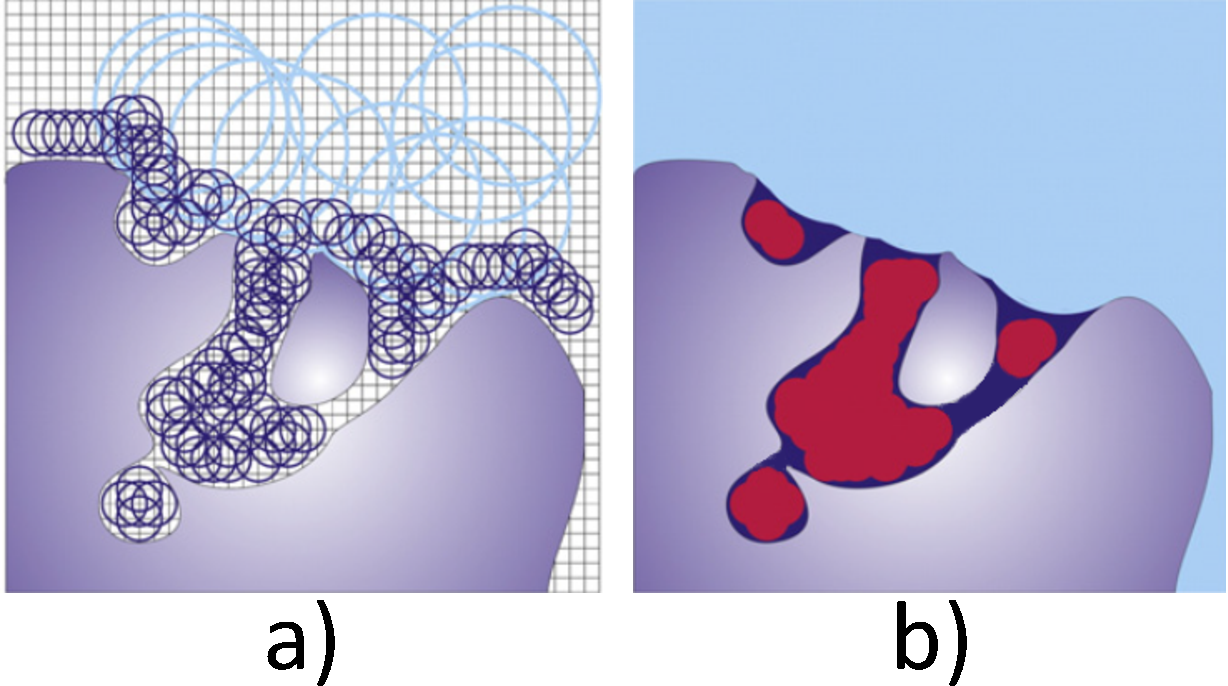
\includegraphics[width=\linewidth]{pictures/rollingprobe.pdf} 
  \caption{a) Rolling probe method. The surface and inner voids of the protein are defined by the placement of probes (large for surrounding and small for voids) in each point of the grid. b) The identified volumes are divided into the protein surrounding (light blue), and internal voids (dark blue), while undetected internal volumes are white. c) HOLLOW represents identified voids using the dummy atoms fitting these voids (red spheres). d) 3V represents detected internal void by voxels (red squares). Image adapted from \cite{brezovsky2013software}.}
  \label{Fig:rollingprobe}  
\end{figure} 

Accuracy of grid-based algorithms strongly depends on the resolution of the voxel grid. At the same time, high resolution of the grid leads to high memory demands of these algorithms. \textbf{Voronoi-based} algorithms in combination with \textbf{path analysis} address these drawbacks by utilizing Voronoi diagrams to subdivide the 3D space of protein structure (see Figure \ref{Fig:voronoi}). Each atom of the protein forms a center of Voronoi cell. The edges are then evaluated by cost function, which assigns the value based on distance of the edge from the cell centres (i.e. atom centres). Then, Dijkstra's algorithm is used on the edge graph to find the best path from the active site towards protein surface. 

\begin{figure}[H]
  \centering
  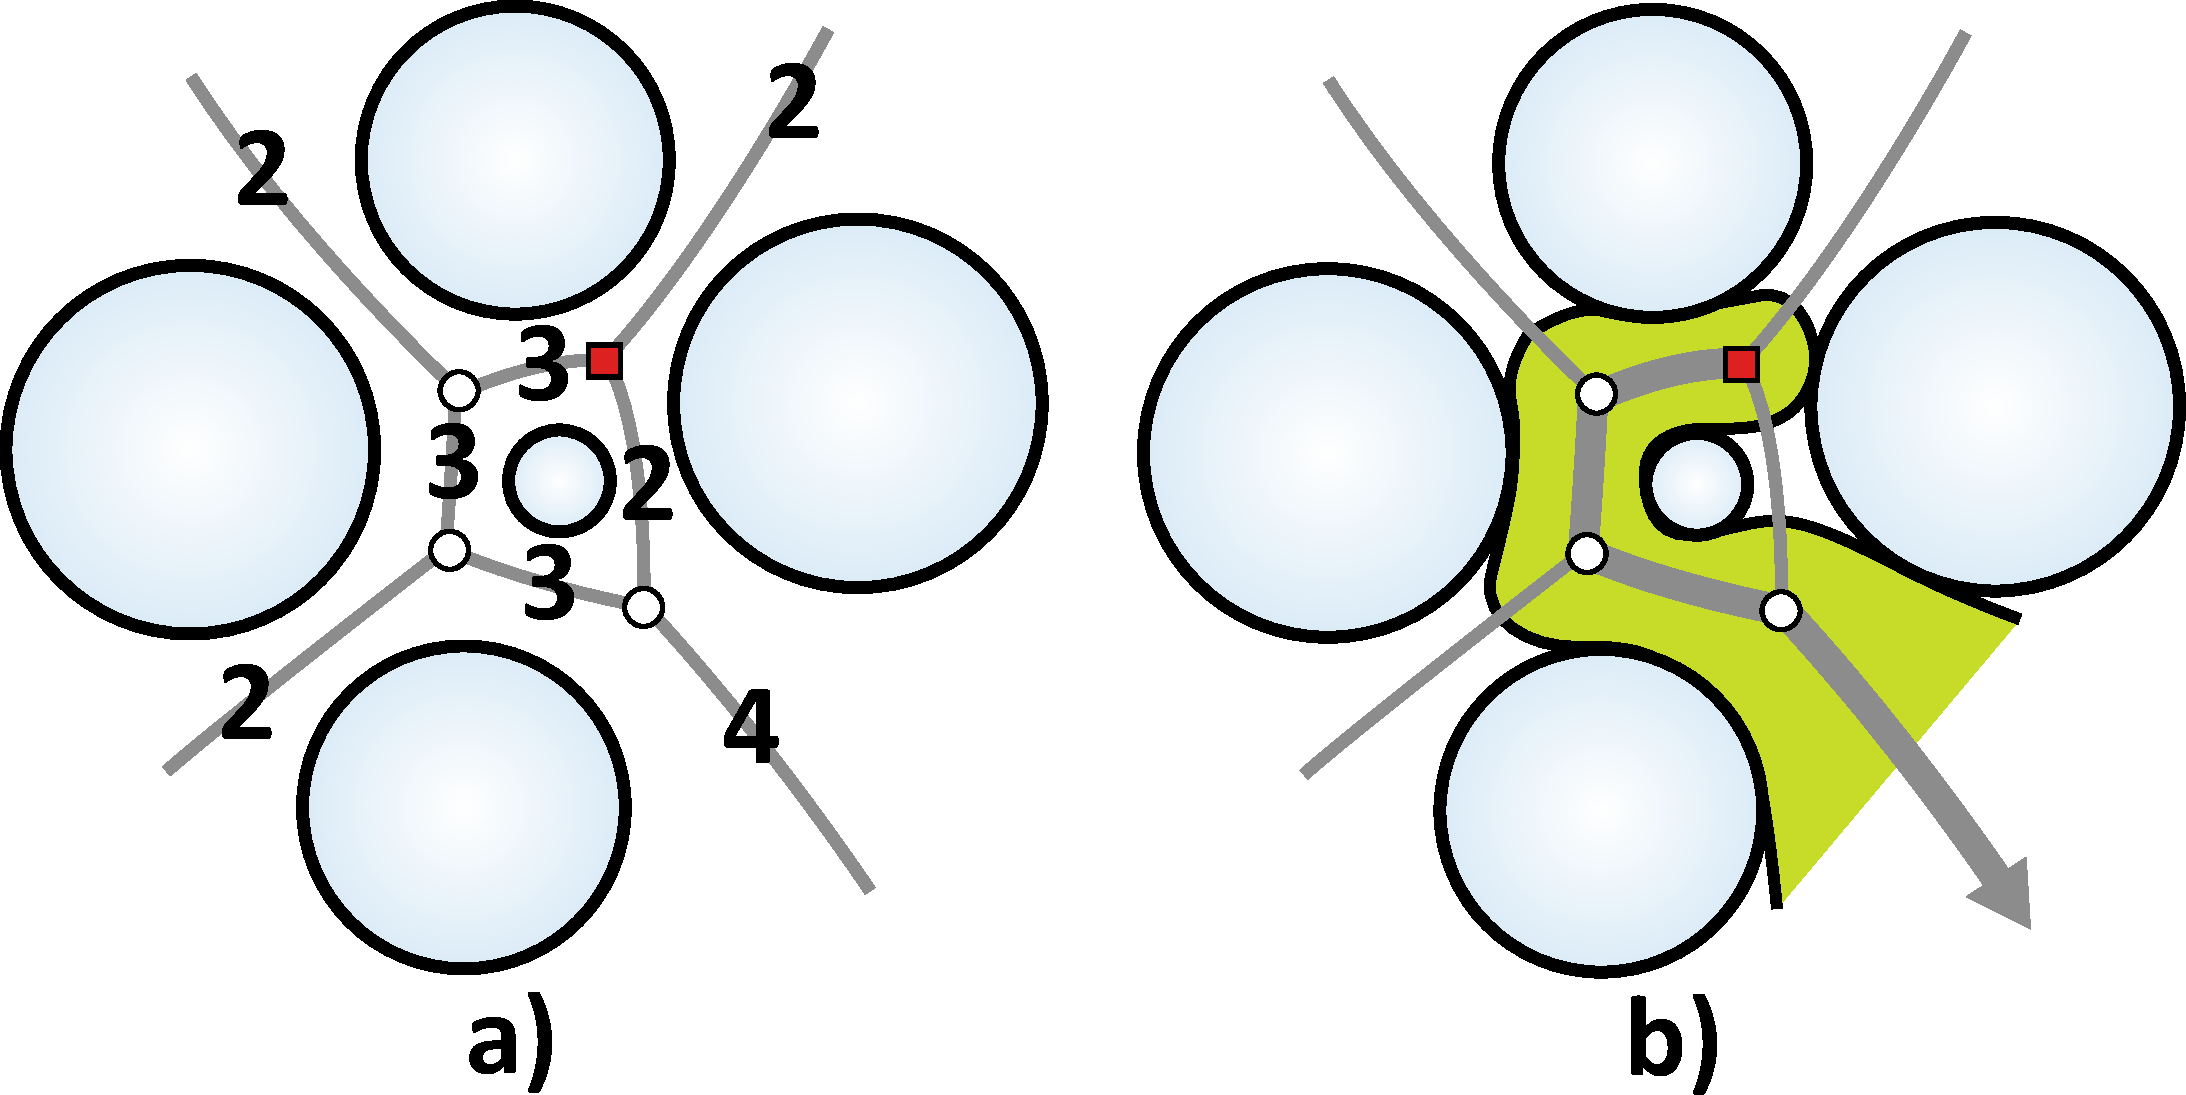
\includegraphics[width=0.6\linewidth]{pictures/voronoi.pdf} 
  \caption{Example of Voronoi-based tunnel detection. a) Evaluated edges. b) Path with highest score found by Dijkstra's algorithm. Red square indicates active site. Image adapted from \cite{caver20}}
  \label{Fig:voronoi}  
\end{figure} 

This principle is used in MOLE~\cite{Petrek2007MOLE} and by Medek et al.~\cite{caver20}. MolAxis~\cite{Yaffe2008MolAxis} increases the precision of this algorithm by approximating atom radii, which previous approaches omitted.

While all these approaches offer a solution for static molecules, CAVER 3.0~\cite{caver30} extends them and allows for detection of tunnels taking into account the movement of the protein. It computes tunnel paths for each time frame of MD simulation. Than the corresponding paths are clustered. Thus it is possible to track the evolution of the tunnels in time.

\subsubsection{Path analysis algorithms}
HOLE \cite{Smart1996Hole}
CHUNNEL \cite{Coleman2009CHUNNEL}
POREWALKER \cite{Pellegrini2009PoreWalker}
 




CAST \cite{liang1998anatomy}

ligand md simulations

\section{Protein-Protein Interactions}
